\documentclass[man]{apa2}
\usepackage{pslatex}
\usepackage{amssymb}
\usepackage{graphicx}
\usepackage{color}
\usepackage{covington}
\usepackage[usenames,dvipsnames]{xcolor}

\title{
%Pragmatic contrast helps preschoolers learn category structure\\
%Pragmatic inferences as a route to learning category structure\\
Knowledge transmission through pragmatic inference in preschool children}

\twoauthors{Alexandra C. Horowitz}{Michael C. Frank}
\twoaffiliations{Department of Psychology, Stanford University}{Department of Psychology, Stanford University}


\abstract{Children learn many instances of cultural norms through direct instruction (e.g. ``red lights mean stop''), but not all conventional knowledge is stated explicitly.  We investigate the hypothesis that children infer generalizable information about the world pragmatically, by making inferences from speakers' descriptive word choices.  We introduced preschoolers to picture triads: an exemplar of a novel category as the base, and then two options that varied from it either by size or by a binary feature. We described the exemplar using either a size term or another polar adjective (e.g., ``this is a [small/broken] tibu''), and asked children which of the two pictures they thought other category members looked like.  In Experiment 1, we used a supportive framing that signaled that the description was contrastive and found that children reliably inferred the property typical of the category.  In Experiment 2, children's performance was reduced when the contrastive framing was removed, but partially restored via a pre-exposure to the relevant adjective pairs. In Experiment 3, a free-response task, children spontaneously produced relevant property contrasts for both size and feature terms.  Our findings suggest that preschoolers can learn about a novel category from a single exemplar---and not just about what that category is, but also what it isn't. More generally, sensitivity to why speakers choose to make particular production choices may allow children to learn efficiently about the world around them. 


% In Experiment 3, we read children a book that highlighted opposite pairs before the task, and this exposure moderately boosted their performance. Preschoolers thus can learn about a novel category from a single exemplar---and not just about what that category is, but also what it isn't. More generally, sensitivity to why speakers choose to describe the world the way they do may allow children to learn efficiently about the world around them. 

~\\

Keywords: pragmatics; language development; adjectives; cultural learning, social inference; production}

\shorttitle{Learning through pragmatics}
\rightheader{Learning through pragmatics}

\acknowledgements{Special thanks to the staff and families at the Bing Nursery School and the Children's Discovery Museum of San Jose. This work supported by a John Merck Scholars Fellowship and ONR grant N00014-13-1-0287. Earlier versions of this work were presented to the Cognitive Science Society in \citeA{horowitz2012} and \citeA{horowitz2014}.

~\\

\noindent Address all correspondence to Alexandra C. Horowitz, Stanford University, Department of Psychology, Jordan Hall, 450 Serra Mall (Bldg. 420), Stanford, CA, 94305. Phone: 650-721-9270. E-mail: \texttt{ahorowit@stanford.edu}}

\begin{document}

\maketitle                            


\section{Introduction}

Children learn some important cultural information through explicit instruction (e.g., ``put the fork on the left of the plate'') and generic statements (``forks go on the left''), but not all norms are stated directly. Sometimes information is implicit in \emph{how} a statement is made. For example, if a parent says, ``that's a salad fork,'' he is implicitly conveying that forks vary in the foods they are intended for (and that most other forks are likely used for non-salad items). More broadly, the way we describe the world can reveal to a perceptive observer all sorts of biases about what we find notable, interesting, or generally worthy of comment---and such biases can in turn act as signals about our knowledge of the world. Are children able to use these implicit signals for learning? 

We focus on contrastive word choices, as in the ``salad fork'' example. Contrastive word choices---the way we use labels and their modifiers---can help identify a speaker's intended referent in the current context (selecting the desired fork) but can also jointly signal generalizable knowledge (forks are associated with meal courses). In the current study, we investigate the idea that adults and children may learn generalizable knowledge via inferences about why speakers choose a particular word to convey a message. 

We test this hypothesis using a simple case study: learning to generalize novel words via minimal contrastive descriptions. To motivate this case study, we begin by discussing two bodies of research: first, work on children's ability to learn about the world from language, and second, work on their ability to reason about the knowledge and beliefs underlying other agents' actions (both non-linguistic and linguistic). This work motivates our current studies: Three experiments investigating preschoolers' generalizations about unseen category members based on speakers' word choices. 

\subsection{Learning from others' explicit statements}

Although learning from the world directly is a very powerful method for acquiring knowledge \cite{gopnik2012b}, there is no way that even the most precocious child-scientist could reconstruct an adult's knowledge from direct experience alone \cite{shafto2012,harris2012}. Instead, children's knowledge comes from a mixture of direct experiences and knowledge transmitted by others. 

Language in particular is an extremely powerful source of information about the world. From the time children begin to speak, they understand that language is used to communicate information \cite{vouloumanos2012,martin2012}. They expect speakers of the same language to use conventional names for conventional meanings \cite{clark1987, markman1988, diesendruck2005}, but learn to recognize that individual knowledge such as facts about objects may not be shared \cite{diesendruck2001}. They also show early knowledge that language can communicate about information that goes beyond the here-and-now \cite{saylor2007,ganea2007}. This early, foundational set of assumptions---that speakers will use language in consistent and communicative ways to convey (relatively) abstract knowledge---is critical in allowing children to use language to learn. 

While some language describes the particulars of the world (e.g., ``the salad fork is on the outside''), other statements provide more general information that applies across situations (``salad forks go on the outside''). Generic language---cued in a number of ways, including the use of a bare plural (``salad forks'') in the previous example---is a particularly powerful method for conveying such information \cite{leslie2008}. Children can use generic language to infer general properties quite early. \citeA{gelman2003} introduced 2--5 year-old children to a a picture (e.g. two penguins) and contrasted questions like  ``Can birds fly?'' (generic) and ``Can these birds fly?'' (non-generic), and found that all age groups distinguished generic from non-generic statements. Children's sensitivity to framing cues leads them to make different assumptions from generic statements (e.g. ``goats can climb trees'') than non-generic statements (e.g. ``this goat can climb trees''). They are more likely to believe that information stated generically is  conceptually and functionally central and more widely-known \cite{cimpian2009, cimpian2010, cimpian2012}, though also recognize that generic statements may allow more room for variability than non-generic statements. Overall, generic language provides an important route for information transmission.
  

%Children's sensitivity to generic framing leads them to make different assumptions from generic statements (e.g. ``goats can climb trees'') than non-generic statements (e.g. ``this goat can climb trees''). They are more likely to believe that information stated generically is  conceptually and functionally central and more widely-known \cite{cimpian2009, cimpian2010, cimpian2012}, though also recognize that generic statements may allow more room for variability than non-generic statements. Overall, generic language provides an important route for information transmission.

In some contexts, generic language is not even necessary: The simple use of a label or even the use of a broader set of communicative cues---child-directed speech, direct gaze, or pointing---may signal that a speaker is presenting information that is relevant to a kind, category, or practice \cite{csibra2009, butler2012}. One striking example of the role of labeling comes from a study in which \citeA{rakoczy2008} introduced 2- and 3-year-old children to a game featuring an action called ``daxing.'' Children then saw a character perform a different action and label it daxing or not.  Both age groups were more likely to protest the new action when it violated their expectations about the meaning of daxing than if it was unlabeled, and they were more likely to provide explicitly normative protests (e.g. ``It doesn't go like that'') than imperative protests (e.g. ``Use the stick'') by age 3. Providing a label for the action led children to expect and enforce that the action was specific and inflexible to other interpretations.  

In fact, preschoolers find it very difficult \emph{not} to believe what they are told.  Three-year-olds can discount inconsistent evidence conveyed through physical markers (e.g. they can learn that an agent purposely places a sticker on the wrong cup, and select the opposite), but they have a much harder time discounting verbal evidence from an unreliable speaker in the same scenario. Even after telling children the \emph{wrong} location consistently, they still look for the hidden item where the speaker says \cite{jaswal2010}.  When given the option to choose between two potential informants, however, preschoolers can recognize which speaker is more accurate and prefer to trust that speaker \cite{pasquini2007}, retaining this preference even after a time delay \cite{corriveau2009}.  Children tend trust verbal information, but privilege accuracy when they can.

To summarize: Explicit linguistic transmission is a powerful and important source of general information about both the specific and the abstract. From an early age children are able to make use of this information, recognizing a number of different cues to the generalizability of the information in a particular statement. We next turn to work on children's ability to make inferences about the unseen causes of actions, both linguistic and non-linguistic.


\subsection{Inferences about others' actions}

% Our work is based on the idea that children make rational inferences about people�s actions.  

In nearly all of the work reviewed above, a parent, teacher, or experimenter presents the relevant information explicitly, via a demonstration or explicit utterance. But a parallel line of work suggests that children and even infants are able to make inferences about the \emph{implicit} sources of both linguistic and non-linguistic actions. This literature is critical for motivating our hypothesis---that such inferences might not just inform guesses about particular agents' knowledge, abilities, preferences, or desires, but that they might also be a source of information about the world more generally. We begin by discussing work on non-linguistic actions and then move on to linguistic (pragmatic) inferences.

\subsubsection{Inferences about others' non-linguistic actions}

By their first birthday, babies appear to make inferences about the constraints and unseen motivations that underly actions, even in very stripped-down displays.  For example, they look longer when a shape that previously jumped over a wall toward another shape continues on the same path when the wall is removed (an action goal) instead of moving directly toward the shape (an end-state goal; \citeNP{gergely1995}. This result is part of a broader body of work suggesting that infants expect agents to act rationally to achieve (inferred) outcomes most efficiently \cite{csibra1998, gergely2003}. In other words, very young children appear sensitive not only to agents' particular actions, but also to the presumed purpose for these actions. 

Further evidence that children actively reason about agents' goals and the constraints on their actions comes from their responses to different sampling contexts. For example, infants are surprised when a random sample is not representative of the overall distribution, but not if it is intentionally sampled \cite{xu2009}.  They can also reevaluate the likelihood of sampling when physical constraints make it more difficult for those items to be sampled (e.g., balls that stick to velcro, \citeNP{denison2010b}).  They can even infer a preference based on non-random sampling \cite{kushnir2010}. This last example is particularly interesting, because it reflects a case in which the children are apparently learning about the agent's general preferences as a statistical inference about the generating cause of a series of individually-ambiguous actions. 

Young children can also consider sampling conditions to make inductive inferences about general properties of objects.  
% Not only can babies infer the likely compositions of populations and probabilities to achieve preferences, but they can also consider evidence and context to make predictions about category members.  
In an experiment by \citeA{gweon2010}, fifteen-month-olds saw a series of blue balls squeaking and then were presented with the opportunity to squeak a slightly different (yellow) ball. Depending on the sampling procedure for the evidence they saw, the children made different generalizations. If the blue balls were sampled from a box of blue balls (implying that they were randomly sampled), the children more likely to think that a yellow ball would also squeak. If the children saw the blue balls picked out from a box of mostly yellow balls (where presumably the blue balls were less likely to be picked randomly, and thus were more likely to be intentionally selected for the demonstration), they thought the yellow balls were less likely to squeak.  
% Children�s sensitivity to not just the evidence, but the conditions under which it is produced appears to guide their expectations about how to extend this knowledge. They appear to go beyond the specific situational information to incorporate cues into a more sophisticated interpretation about the social world.
Taken together, these findings support the idea that children make inferences about agents' actions and work backwards to infer the perceived norm or state of the world that motivates these actions. 


% By one year of age, babies demonstrate sensitivity to the composition and conditions of sampling, and use these cues to make inferences about broader populations.  They incorporate both statistical and social information to form expectations about the world. 

\subsubsection{Inferences about others' linguistic actions}

The inferences described above show a striking similarity to a quite different kind of inference: pragmatic inferences in language comprehension  \cite{shafto2012}. In classic examples of pragmatic inference, language comprehenders reason about the generating causes of a (linguistic) action and about the constraints on the agent. In Grice's \citeyear{grice1975} classic example, the recommender who declares that his student has good penmanship is choosing an action that completes his goal---write a letter that is maximally informative about the student---while complying with the restrictions on his actions---be truthful, don't say anything negative. Grice famously formalized these tradeoffs in reasoning about linguistic actions as a series of maxims---be truthful, informative, relevant, and clear---and derived a number of important linguistic phenomena from their intersection. For example, on the basis of the above letter of recommendation, a reader of the letter can make the \emph{implicature} that the speaker does not believe the applicant has any other positive qualities (or else the letter writer would have mentioned them). Since Grice's initial formulation, a number of other theories have described the exact tradeoff that governs speakers' actions differently \cite{horn1984,sperber1986,clark1996,levinson2000}, even as they have preserved the basic idea of pragmatic inference as action understanding.

Are children able to make such inferences as well?  Initial work suggested that they might show deficits in this kind of pragmatic language understanding through age five or even later \cite{noveck2000,papafragou2003}: when presented with a situation where three of three horses jumped a fence, children would judge the utterance ``some of the horses jumped over the fence'' to be a felicitous description. The necessary pattern of reasoning to make the implicature in this case would be that if the speaker said ``some,'' she probably couldn't have truthfully uttered the stronger term ``all.''

A more recent body of work suggests that these deficits are specific to particular linguistic phenomena---in particular, scalar implicatures using quantifiers like ``some'' and ``all'' \cite{barner2011,katsos2011}. One interpretation of these failures is that children have trouble holding in mind and contrasting the alternative statements ``some'' and ``all.'' This \emph{alternatives hypothesis} makes a number of predictions that have now been tested. First, children have difficulties with even non-pragmatic interpretations that require considering these alternatives (e.g., reasoning about what ``only some'' means; \citeNP{barner2011}). Second, exposure to alternatives increases levels of implicature \cite{skordos2014}. Third, in contexts where alternative meanings are more explicit (e.g. pictured as alternatives in a forced-choice), children perform better \cite{miller2005,stiller2014}. Thus, children appear to be more pragmatically-sophisticated than some accounts have given them credit for.


\subsection{Our current study}

Given that children are able to make a number of sophisticated inferences about the basis for both linguistic and non-linguistic actions, we ask whether these inferences can provide a method for the transmission of information. In particular, we investigate preschoolers' ability to infer information about a general class from the specific production choices speakers make. For example, labeling a novel item as a ``tall blicket'' gives information not only that this item is a tall blicket, but it also suggests that height is a relevant variable property to blickets, and that other blickets may be short. 

As in our ``tall blicket'' example, we focus on adjectives as a case study.  Because adjectives are optional modifiers, they can be included in an utterance to draw contrasts between an intended referent and its unintended alternatives. Therefore, working backwards, if the listener does not know what the unintended alternatives are, the inclusion of an adjective could convey important information about contrasts that are relevant for a particular category or comparison. In this way, an optional modifier could provide important general information about a property of interest and its pragmatic alternatives.

Children show evidence of making contrastive use of prenominal adjectives (e.g. ``red car'') in their real-time language comprehension by age 3 \cite{fernald2010}, and in more complex referential communication task by kindergarten \cite{nadig2002}. Work to date has focused on how adjectives are used in context, however.  In contrast, here we examine a novel question, asking how adjective use can help listeners infer \emph{what the context is}.  In other words, we ask whether children can infer that adjective use conveys not only information about the referent, but also information about contrastive properties of non-present category members.

In the three experiments below, we use a simple triad task to investigate preschoolers' inferences about adjective use and category membership.  We introduced children to a novel shape, followed by two similar shapes: one that differed from the first only by size, and the other that differed from the first only by a different polar feature (e.g. wet/dry). For convenience here and below, we refer to this distinction as ``size'' vs. ``feature.''  We described the first shape using either a size or feature adjective, and asked children to generalize what they thought other category members looked like.  

If children generalize from the exact language they hear, then they should expect other category members to share the same property (i.e. if the first shape is labeled as ``small,'' then they should select that other shapes also look small). If they generalize from the \emph{property choice} conveyed from the speaker's adjective use, then they should instead select the property \emph{contrast} (i.e. hear ``small'' and select the shape that's bigger).  In Experiment 1, we found that preschoolers' contrast inferences increased across the preschool years, and were reliably above chance for both size and feature terms for 3.5 -- 5-year-olds.  
In Experiment 2, performance decreased in a more stripped down version of the task with reduced contrastive framing, but increased exposure to contrasts after reading a book of opposites before the task moderately recovered performance. In Experiment 3, children generated relevant contrasts the majority of the time in a free-response adaptation of the task.  Overall, we see that preschoolers are sensitive to speakers' use of adjectives as a cue to implied dimensions of contrast. 
%\cite{schmidt2012}

\section{Experiment 1}

We wanted to investigate whether preschoolers are sensitive to information about the world that is pragmatically conveyed through speakers' word choices. We first investigated preschoolers' sensitivity to implied contrasts using familiar scalar properties. We reasoned that children may be more likely to infer contrast information when they are able to recognize that the adjective used is a member of an opposite pair (e.g. tall--short). We designed a task in which the choice of adjective was the only informative cue to implicit referential contrast. If children use adjective information to generalize, they should identify other category members by matching this property. If they use adjective information to make inferences about implied contrasts, they should identify other category members by whether they contrast along the stated dimension. We found that young 3--year--olds were unable to systematically recognize category membership through speakers' adjective choices, but age 3.5, children showed sensitivity to implicit dimensions of contrast contained in word choice. By age 5, children made contrast inferences at similar rates to adults. 

\subsection{Methods}

\subsubsection{Participants}

We recruited a planned sample of 96 children into four age groups: 3.0--3.5 years (n=24, mean age 3;3), 3.5--4.0 years (n=24, mean age 3;9), 4.0--4.5 years (n=24, mean age 4;3), and 4.5--5.0 years (n=24, mean age 4;8).  About half of the sample was recruited from the Bing Nursery School at Stanford University (n=52) and half was recruited from the Children's Discovery Museum (CDM) of San Jose (n=44), divided approximately evenly across age groups.
  
Children were tested individually in a quiet room at either the nursery school or the museum. At the CDM, parents accompanied children and sat either next to or behind the child, and children received a sticker and a certificate for their participation. If siblings also attended, they were provided quiet toys or activities such as coloring or reading during the testing prodecure. Parents were asked to fill out a short demographic form about their children's language background.  Only children who were reported to hear English at least 75\% of the time were included in the final sample.  Eight participants were excluded from analysis based on this criterion\footnote{In our partnership with the CDM, we invite any interested visitors to participate in our studies rather than prescreening children to meet our language requirements or counterbalance all demographic factors \cite{callanan2012}. Bing Nursery School is an English language preschool, and children included in the sample were fluent speakers of English. Children from Bing Nursery School and the CDM are roughly equated demographically in terms of language exposure, ethnic backgrounds, and parental education, as reported by parents from each location.  Both locations were mainly composed of educated middle class families.  We tested for effect of location, and found no differences across children tested at either location.}.  An additional two participants were excluded for not completing all four experimental trials. 

%\footnote{Some variability in age and gender counts across locations arises from our commitment to recruit inclusively at the Children's Discovery Museum. In our partnership with the Children's Discovery Museum, we invite any interested visitors to participate in our studies rather than prescreening children to meet our language requirements or counterbalance all demographic factors \cite{callanan2012}.}


We also ran a comparison group of 128 adult participants through Amazon's Mechanical Turk online crowd-sourcing service.  Participants were all reportedly native English speakers and residents of the United States. They were informed that the task was designed for children.  Three participants were excluded for failing to complete the task.  

\subsubsection{Materials}

Children were read a storybook with colorful clipart images.  Each child participated in two training trials and four test trials.  Training trials featured three pictures of familiar items, only two of which shared a contrast property (e.g. chocolate milk, plain milk, and orange juice).  For the test trials, children were shown sets of three unfamiliar images: a novel exemplar shape as the base followed by one image that differed from the exemplar only by size, and one image that differed from the exemplar only by a feature contrast (e.g. broken versus unbroken) (See Figure \ref{fig:inanimate_demo}). The named size contrasts were \emph{small} (vs. big), \emph{long} (vs. short), \emph{tall} (vs. short), and \emph{short} (vs. long).  The named feature contrasts were \emph{broken} (vs. unbroken), \emph{pointy} (vs. smooth), \emph{dirty} (vs. clean), and \emph{wet} (vs. dry).  To ensure that children were familiar with the contrasts used, a posttest of pictures exemplifying each of these properties was included in a posttest.  Children were able to recognize the contrasts used in our task, with average accuracy of 90\% for 3--3.5 year--olds, 95\% for 3.5--4.0 year--olds, 96\% for 4.0--4.5 year--olds, and 98\% for 4.5--5.0 year--olds.  

The task was adapted to an online format for adults.  Adults viewed a single trial composed of one of the picture triads. The same expressions read to children were written for adults to read on their own. 

\begin{figure}[t]
  \begin{center} 
    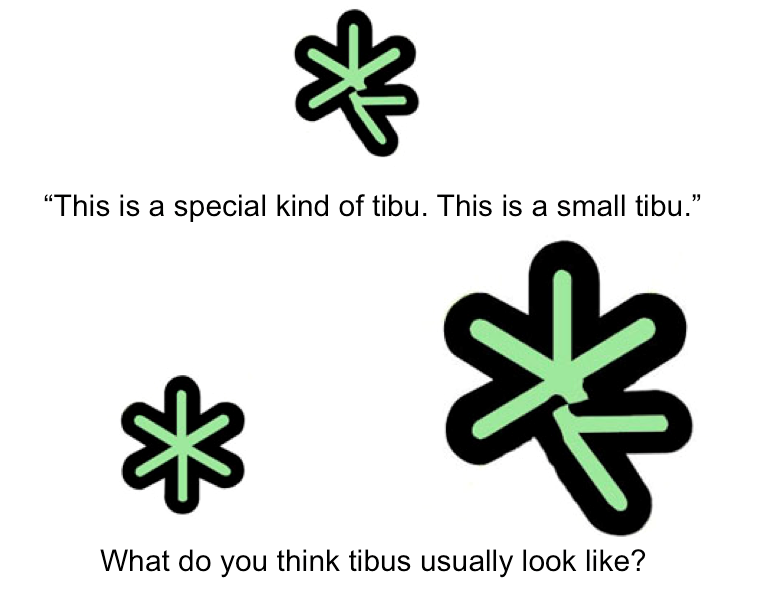
\includegraphics[width=4in]{figures/inanimate_demo.png} 
    \caption{\label{fig:inanimate_demo} Example of a test trial for Experiment 1a.  Participants were introduced to a base exemplar shape (top) described with either a size or feature adjective.  They were then shown two images, one that differed from the exemplar by a feature (left) and one that differed from the exemplar by size (right) and were asked to point to which picture they thought was also a member of the same category. } 
  \end{center} 
\end{figure}	



\subsubsection{Procedure}

The experimenter read the storybook with children individually in a quiet room at either Bing Nursery School of the San Jose Children's Discovery Museum.  At the museum, parents accompanied children and sat either next to or behind the child.  Siblings were sometimes also present, and were offered quiet activities such as coloring or reading. 

To begin the book, children were introduced to a character named Allen the Alien who was visiting planet Earth.  Children then participated in two training trials containing familiar items to teach Allen about some things on Earth and get children used to the study design.  Training trials featured adjectives other than those used in critical trials, and training pictures displayed only one relevant contrast choice.  For example, children were shown a picture of chocolate milk followed by two pictures, one of plain milk and one of orange juice.  Children were told, ``This is a special kind of milk.  This is \emph{chocolate} milk.  What does milk usually look like?  What does most milk look like?" and prompted to point to the picture.  On the rare occasion that children answered incorrectly, the experimenter repeated the statements and encouraged children to point to the correct picture until they answered correctly.  

After the training trials, children participated in four test trials.  For each test trial, children were shown a picture of a single base exemplar (e.g. a small broken tibu, see Figure \ref{fig:inanimate_demo}) and told something about it, e.g. ``This is a special kind of tibu.  This is a small tibu."  They were then shown two similar pictures, one that differed from the exemplar only by size (i.e. a big broken tibu) and one that differed from the exemplar only by a feature (i.e. a small fixed tibu), and were asked ``What do you think tibus usually look like?  What do you think most tibus look like?" They were prompted to select one of non-exemplar images.  Two of the four trials used size adjectives (e.g. ``This is a small tibu") and two of the trials used feature adjectives (e.g. ``This is a broken tibu"). The order of trial items varied across two lists, each of which was counterbalanced for adjective type and picture order.  Adjectives were focused using contrastive stress.  The experimenter averted her gaze while children pointed to their responses.  Responses were coded online and double-coded offline using a video recording of the testing session.  The task took about ten minutes to complete. 

Adults were randomly assigned to a single test trial.  Picture type, side, and adjective were counterbalanced across participants.  Adults indicated their response using a radio button below their image selection.  Participants were paid 25 cents for completing the task, which took about two minutes to complete. 

\subsection{Results and discussion}

%Responses were coded as correct if participants selected the shape that differed along the referenced dimension.  In other words, we considered a response to be a correct contrast judgement if the participant selected the shape that differed by feature in feature adjective trials (e.g. heard ``broken'' and selected the shape that was unbroken), and differed by size in size adjective trials (e.g. heard ``small'' and selected the shape that was big).  


We categorized a response as a correct contrast inference if children selected the item that differed from the exemplar along the referenced dimension (i.e. they chose the short item if the exemplar was referred to as ``tall", but the clean item if it was referenced as ``dirty").  We found that preschoolers' sensitivity to contrast information implicit to adjective choice increased from ages 3--6 years of age.  The youngest children in our sample did not demonstrate systematic inferences to adjective information; 3--3.5 year--olds selected the adjective match and the adjective contrast at chance levels when selecting another example of a category member with the referent.  However, by age 3.5, children predictively selected the contrasting property to the adjective named.  Within the early preschool years, children appear to gain sensitivity in assessing speakers' word choice information and the implicit contrast information it may contain. 

Overall, we see that, although even the youngest children in our sample were familiar with the adjectives and their contrast alternatives used in our task, children younger than age 3--and--a--half were unable to reliably use adjective information to infer implicit contrast information.  However, children ages 3.5--4.0 were reliably above chance in selecting the contrast property when size terms were used, and marginally above chance when feature contrasts were used.  Children ages 4.0--4.5 and 4.5--5.0 were reliably above chance in selecting the property contrast across both feature and size terms.  The oldest children matched the performance level of adults, who made contrast selections robustly above chance for both adjective types ($p < .001$ in exact binomial tests for feature and size terms). 

We analyzed our results using a logistic mixed model, predicting correct responses as an interaction between age and contrast type with random effects of participant and shape.  Children increasingly made more correct contrast judgments with age ($\beta = 1.51$, $p < .0001$). 
% There was a significant effect of age, such that children increasingly made more correct contrast judgments with age ($\beta = 1.51$, $p < .0001$).   
There was no significant effect of contrast type (feature vs. size adjectives), and there was no interaction between age and contrast type, suggesting that participants across ages did not differ in their responses to different property types.  Overall, these analyses show that children demonstrate an increasing sensitivity to implicit contrast information from adjectives.  

%Adults selected the contrasting dimension more often than chance and at nearly identical rates for both adjective types ($p < .001$ in exact binomial tests for feature and size terms; see Figure \ref{fig:expt1_kidsAdults}).  Our results indicate that participants used the adjective referenced to make inferences about properties of novel category members, suggesting that adjectives are informative indicators of relevant property information to adults.  They were able to consider the labeled property in order to infer that other novel category members are likely to differ along the referenced dimension. 

Adults had no difficulty inferring contrast from adjective use in our task, and preschoolers showed a developmental increase in performance before reaching that of adults by age 5.  Our results indicate that adults and young children are sensitive to the contrastive implications of speakers' use of adjectives.  Rather than selecting the image that matched the named property, adults and children selected the property contrast.  Inferences about relevant implied alternatives may allow listeners to pick up on socially-relevant information conveyed through production choices. 


\begin{figure}[t] 
  \begin{center} 
    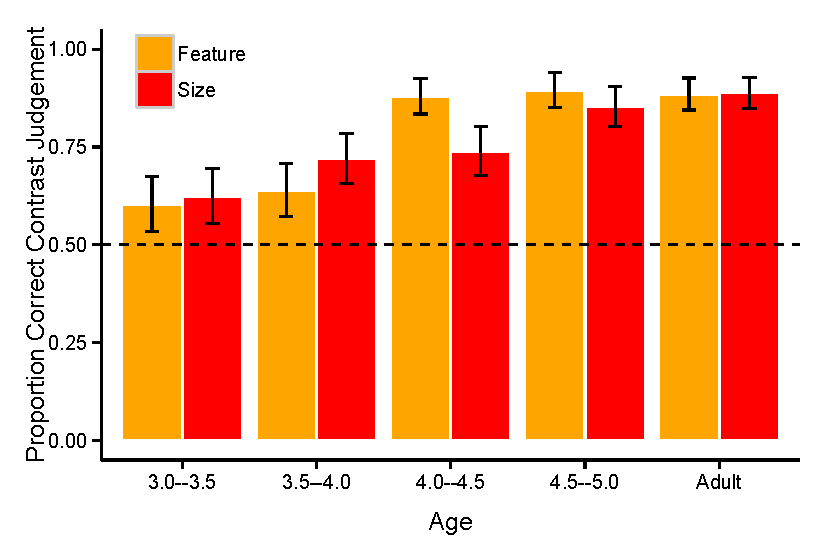
\includegraphics[width=6in]{figures/expt1_kidsAdults.pdf} 
    \caption{\label{fig:expt1_kidsAdults} Preschoolers' and adults� mean proportion correct performance in Experiment 1. Yellow bars depict feature adjective trials and red bars depict size trials. The dashed line represents chance (0.5). Error bars represent standard error.}
    %95\% confidence intervals.} 
  \end{center} 
  % \vspace{-2.0ex} 
\end{figure}	


\section{Experiment 2}

In our first set of experiments, we found that adults consistently made contrast inferences from adjective use, while preschoolers gained sensitivity to how speakers mark relevant property information with age.  They may begin by appreciating that scalar opposites are paired, and that use of one term (e.g. \emph{wet}) implies contrast with its opposite (i.e. \emph{dry}). We next wanted to investigate the robustness of children's contrast inferences for opposite terms.  In Experiment 2, we removed the contrastive framing (i.e. stating that ``this is a special kind of...'' ) to examine children�s sensitivity to adjective use as the only cue to contrast.  We assigned children to one of three conditions: in the \emph{adjective only}, we measured 4-year-olds' and a comparison group of adults' contrast inferences from adjective production alone (e.g. ``This is a tibu. This is a small tibu.''). This change allowed us to examine listeners' sensitivity to implied contrast from scalar terms without the support of other pragmatic cues.  We were concerned that the subtlety of both identifying the adjective as an informative word choice and also inferring category membership based on its property contrasts might be difficult for children to process spontaneously, so we attempted to alleviate this cognitive burden through two priming conditions: in the \emph{paired order} book condition, we read a book of opposites before introducing children to the experimental task to remind them of the contrastive nature of adjectives.  In the \emph{scrambled order} condition, we read the same book of opposite terms to children, but in a scrambled order so that they heard all the same terms but not used as direct contrasts.  Although adults had no difficulty inferring contrast information from adjective use alone, preschoolers had more difficulty, but their contrast inferences improved moderately after reading the opposite pairs book, and slightly less so for the scrambled book.  Children may initially require support to recognize the informative of adjective use before spontaneously making contrast inferences from these word choices alone. 


\subsection{Methods}

\subsubsection{Participants}
A new sample of 144 children was recruited from Bing Nursery School.  Because of the presumed increased difficulty of this task, we recruited children from the older age groups: 4.0--4.5 years (n=72, mean age 4;3) and 4.5---5.0 years (n=72, mean age 4;8).  A third of children in each age group (24 younger 4s and 24 older 4s) were randomly assigned to each of the three conditions (\emph{adjective only}, \emph{paired order} pre-test book, or \emph{scrambled order} pre-test book). 

We also ran a new group of 128 adult participants in the \emph{adjective only} condition on Amazon's Mechanical Turk.  All participants were reported to be US residents and native English speakers.  They were informed that the task was designed for children.  Seven subjects were excluded for failing to complete the task. 

\subsubsection{Materials}
Stimuli were identical to Experiment 1 with the addition of one of two separate training books read prior to the testing procedure.  Each training book consisted of clip art images of familiar items depicting the size and feature contrasts portrayed in the test book. The training books were identical except for the ordering of the pages. In the \emph{paired} condition, opposites were paired so that scalar contrasts were viewed simultaneously and stated consecutively (e.g. ``Here is a small teddybear.  Here is a big teddybear.'')  In the \emph{scrambled} condition, the orders of the pages were mixed up so that consecutive pages conveyed a size and a feature description, and opposites never appeared together (e.g. ``Here is a small teddybear.  Here is a wet car.'') Sample images are presented in Figure \ref{fig:book_demo}.


\begin{figure}[t] 
  \begin{center} 
    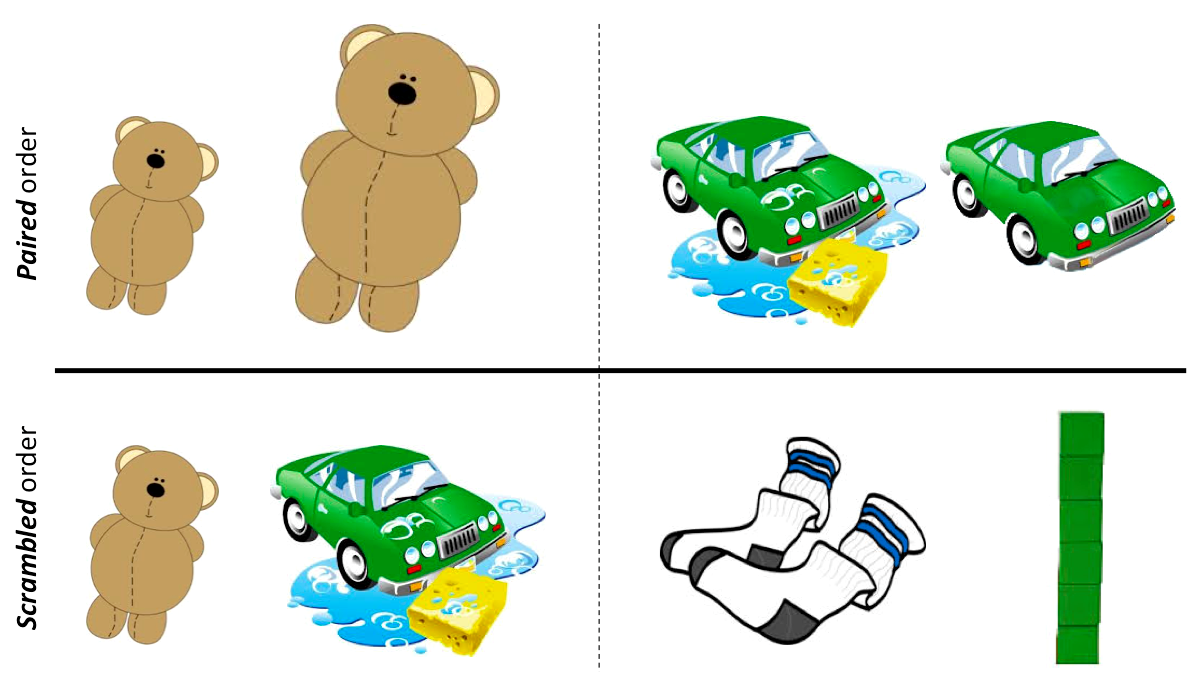
\includegraphics[width=6in]{figures/aliens_book_demo.png} 
    \caption{\label{fig:book_demo} Sample images from the adjectives naming books used in Experiment 3.  The top row depicts two pages of the \emph{paired} condition, in which opposite terms were labeled consecutively (e.g.  ``Here is a small teddybear. Here is a big teddybear.'' and ``Here is a wet car. Here is a dry car.'').  The bottom row depicts two pages of the \emph{scrambled} condition, in which individual opposite terms were interspersed rather than appearing together (e.g. ``Here is a small teddybear. Here is a wet car.'' and ``Here are clean socks. Here is a tall tower of blocks.'').}
  \end{center} 
\end{figure}	


\subsubsection{Procedure}
Procedures for the experimental task were identical to Experiment 1 with the exception that the referential phrase was minimized by removing the phrase ``special kind of'' to reduce contrast cues other than the adjective.  Instead, participants heard only ``This is a [tibu]. This is a [broken tibu],'' isolating the adjective as the only available indicator of category membership.  As in Experiment 1, adult participants were randomly assigned to a single test trial presented online. 

Children in the \emph{paired order} and \emph{scrambled order} book conditions were told that they would be reading two books for the session.  The procedure was identical to that of Experiment 2 with the addition of an adjectives naming book immediately preceding the test book. The experimenter read the adjectives book with children, labeling each picture in a neutral way on each page (e.g. ``Here is a small teddybear. Here is a big teddybear.'').  The books were identical except for the order. Although the properties used in adjectives naming books were the same as those in the test book, no child explicitly noted any connection between the books. 


\subsection{Results and discussion}


\begin{figure}[t] 
  \begin{center} 
    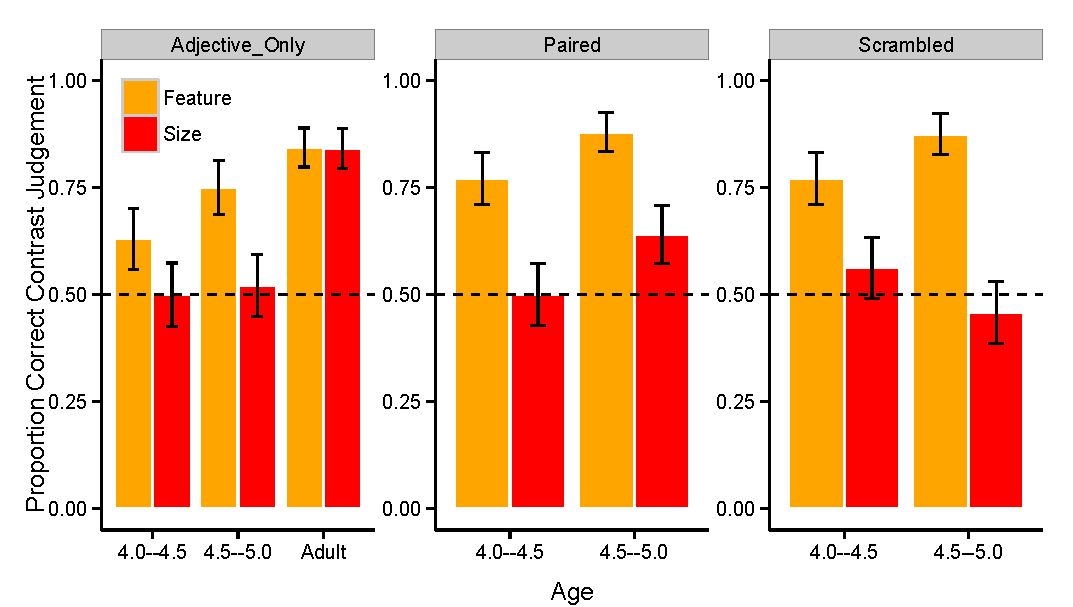
\includegraphics[width=6in]{figures/expt2_kidsAdults.pdf} 
    \caption{\label{fig:expt2_kidsAdults} Results from Experiment 2.  Preschoolers' and adults' proportion correct performance for the \emph{adjective only} condition are shown on the left, followed by preschoolers' performance for the \emph{paired} contrasts (middle) and \emph{scrambled}  contrasts (right) pretest book conditions. The dashed line represents chance (0.5). Error bars show standard error.}
  \end{center} 
  % \vspace{-2.0ex} 
\end{figure}



	
%\begin{figure}[t] 
%  \begin{center} 
%    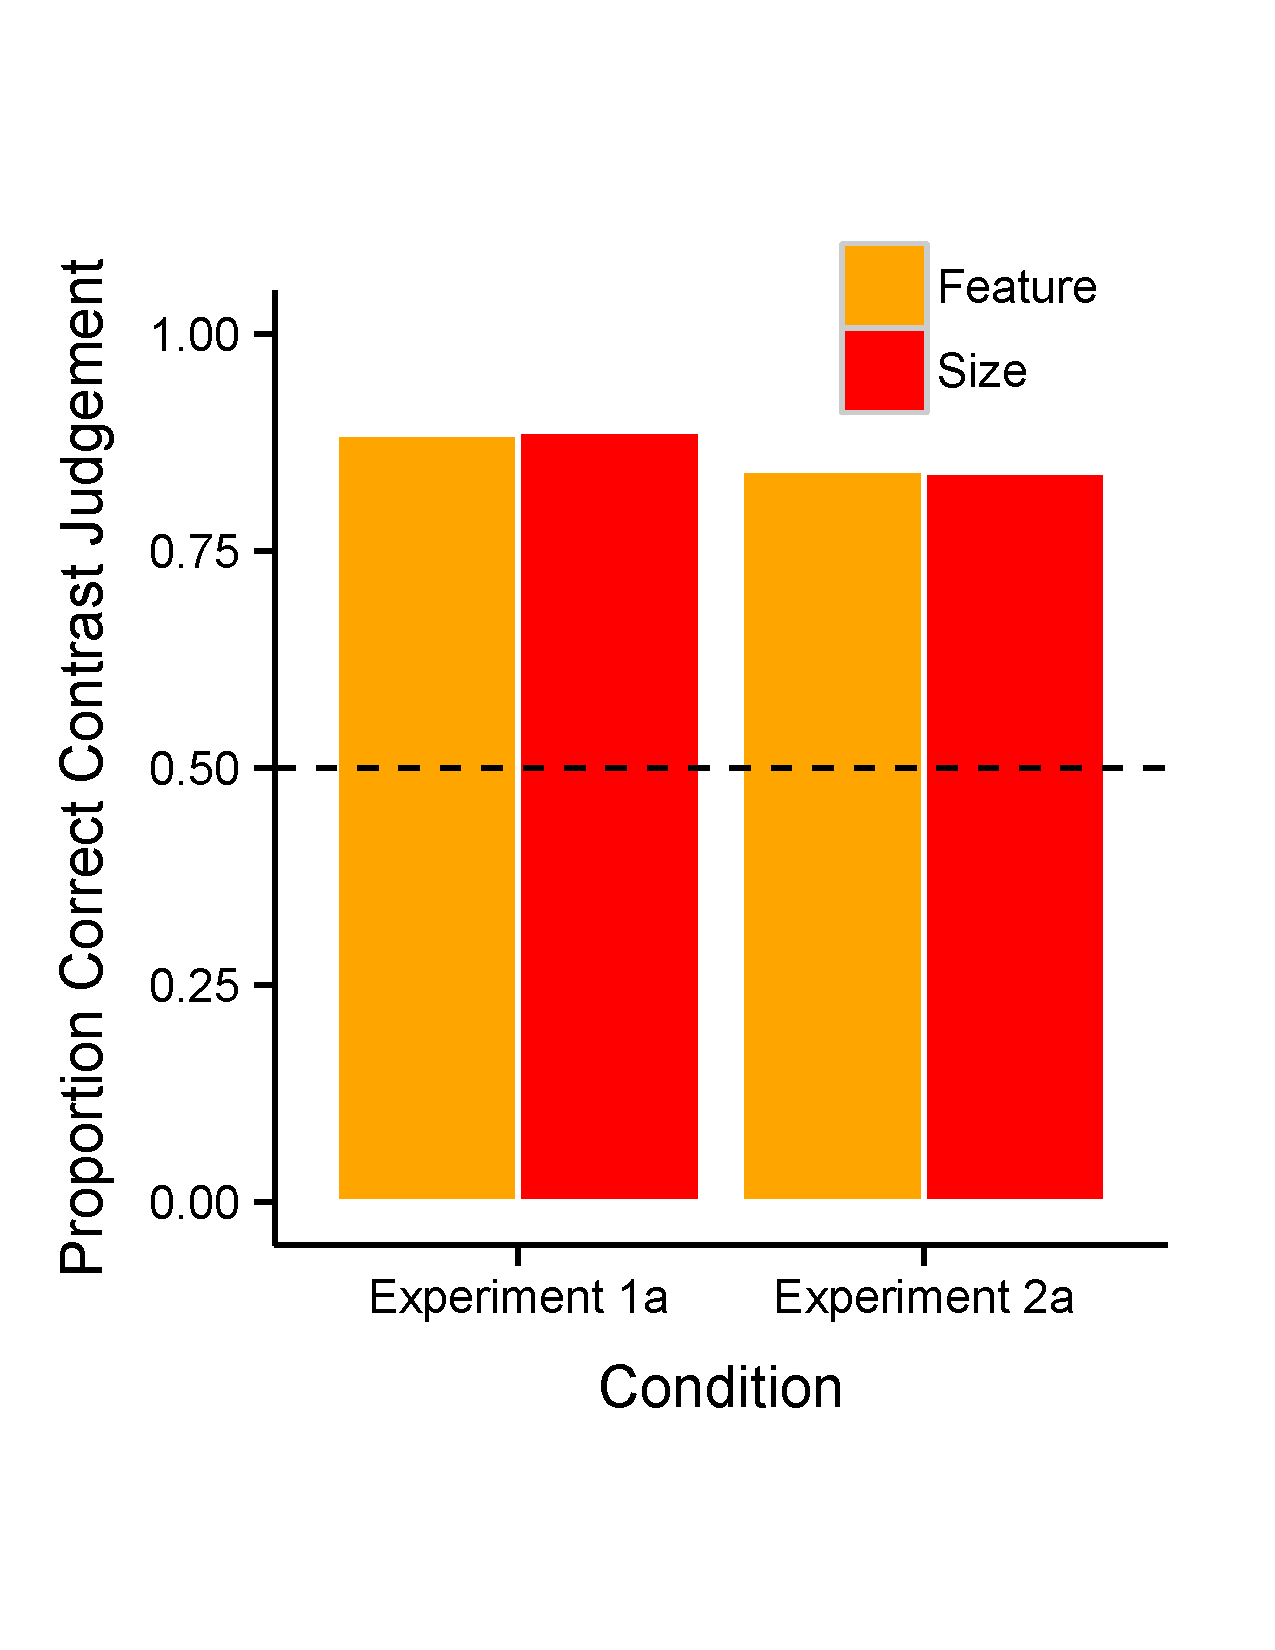
\includegraphics[width=3in]{figures/adults2.pdf} 
%    \caption{\label{fig:adults_plot} Adults' mean proportion correct performance in Experiments 1a and 2a. Feature trials are plotted in yellow and size trials in red. The dashed line represents chance (0.5). }
%    %Error bars represent 95\% confidence intervals.} 
%  \end{center} 
%  % \vspace{-2.0ex} 
%\end{figure}	


Although preschoolers showed increasing contrast selections from adjective use with age in Experiment 1b, they were essentially at chance when the contrastive language framing was removed.  We analyzed our results using a logistic mixed model, predicting correct responses as an interaction between age and contrast type with random effects of participant and shape, and we found no significant effects and no significant interaction. In post-hoc followup tests, older 4s showed a significant feature contrast bias ($p  = .001$, exact binomial test), but this contrast was not reliable in the full model when controlling for participant and item effects, and may have been driven primarily by the ``broken'' and ``clean'' items. Although adults remained attentive to implicit contrast information in both the contrastive language and adjective only framings, children performed substantially worse without the additional linguistic cues to guide their contrast judgements.  

%UPDATE THIS INFO WITH LAST FEW KIDS

As above, we measured the proportion of correct contrast judgments for which participants selected the test picture that differed along the referenced property dimension.  Adults performance was significantly about chance ($p < .001$ in exact binomial tests for feature and size terms) and did not differ by adjective type.  They showed only a slight decrease in performance in this adjective only framing from the contrastive language framing in Experiment 1c (see Figure \ref{fig:expt2_kidsAdults}).  These results indicate that adjective use in our task is a strong indicator of relevant property information of novel category members for adults.  Their nearly equal performance across Experiment 1a and 2a suggests that adjectives provided salient cues to implicit contrast dimensions on their own without the necessity of additional semantic support. 


Increasing preschoolers' access to relevant linguistic alternatives helped older 4s select property contrasts for both feature and size adjectives.  These results suggest that supporting children's abilities to bring relevant alternatives to mind plays a strong role in their pragmatic inferences. Beyond relying on rich semantic framing cues to intended meaning, which are not always available in natural speech, reminding children of different types of modifiers increases their likelihood of forming contrast inferences from adjectives alone. 

Older children selected the contrast property for both feature and size terms more often than chance ($p < .001$ and $p < 0.01$ respectively in exact binomial tests) and younger children for feature terms ($p = .01$ in exact binomial test), though younger children's performance did not differ across feature and size trials.  A logistic mixed model predicting correct responses as an interaction between age and contrast type with random effects of participant and shape revealed no significant effects or interaction, however.

%When we combine results with those of Experiment 2b, we find a three-way interaction between experiment, adjective type, and age, such that older children show improved contrast inferences for size terms only after the opposites book ($\beta = 2.60$, $p = 0.04$).  Increased access to lexical alternatives seemed to help older children reliably select the dimension contrast according to the property.  

Our results from Experiment 2 suggest that exposing children to a book of unrelated pictures with the scalar alternatives used in our test trials helped older children to select opposites more consistently, without any framing cues.  An alternative hypothesis, that the initial book served to train children to always select named opposites, is not supported because we did not see a change in performance for the youngest children.  In addition, anecdotally none of the children remarked on any relationship between the books, even though they conveyed the same adjective properties.  Instead, we believe that the opposites book served to make the lexical scales more accessible to children so that, at least for the oldest children in our task, they could spontaneously infer implicit contrast information from an adjective produced alone.   


%Although children succeeded in forming contrast inferences from adjective with in the contrastive language framing (Experiment 1b), they had difficulty when the adjective was provided on its own without other cues to contrast (Experiment 2b). 


% If children rely on the support of evidence that adjectives imply contrasts with paired alternatives, then they may gain a boost in their ability to make contrast inferences after being reminded of opposite pairs book.  If they 


%In Experiment 3, we provide a test of the linguistic alternatives hypothesis by increasing preschoolers' access to the relevant lexical alternatives.  Before the experimental procedure, the experimenter read a seemingly unrelated book featuring the opposites referenced in the test trials (see Figure \ref{fig:training_demo}).  This exposure to linguistic alternatives boosted older 4-year-olds' contrast selections. 


\section{Experiment 3} 

In Experiments 1 and 2, we found that preschoolers can make contrast inferences from adjective use, but that they may rely on the support of contrastive linguistic framing or a reminder of the contrastive nature of modifiers before recognizing the informativeness of these word choices on their own as adults do.  Although we were able to measure developmental differences in our first experiments, our results are limited to children�s selections in a forced-choice procedure.  In Experiment 3, we wanted to test the extent of children�s more natural responses to adjective use.  We modified our design to examine children�s productions in a free response version of the task.  We told children that, e.g. ``This is a plizzle. There are different kinds of plizzles. This one is a small plizzle. What do you think other plizzles look like?'' Even in this open-ended context, 4-year-olds produced relevant alternatives more than half the time. Our findings suggest that preschoolers spontaneously pick up on pragmatic productive choices to infer implied information about the world. Even without specified alternatives available, preschoolers show strong proficiency at inferring cues and implications from language use. 

\subsection{Methods}

\subsubsection{Participants}

A new planned sample of 24 children (mean age 4;6) were recruited from the Children�s Discovery Museum of San Jose.  Only children reported to use English at least 75\% of the time were included in the final sample.  Two participants were excluded for using less than this amount of English, and one participant was excluded for not producing responses to the experimenter's questions.

\subsubsection{Materials}

We used a similar task design as Experiments 1 and 2, but showed children only a single picture rather than a triad.  We also modified the items to convey more accessible lexical alternatives to children because some of the original items depicted contrasts that were visually salient but perhaps more difficult to articulate (e.g. ``broken'' to ``unbroken'' or ``fixed'').  The named size contrasts used were \emph{small} (vs. big), \emph{tall} (vs. short), \emph{long} (vs. short), and \emph{skinny} (vs. fat).  The named feature contrasts were \emph{hot} (vs. cold), \emph{dark} (vs. light), \emph{wet} (vs. dry), and \emph{open} (vs. closed).  We also ran a posttest to ensure that children were familiar with all of the properties used in the task.  Children successfully identified the contrasts 96\% of the time.

\subsubsection{Procedure}

The experimenter read the storybook with children individually in a quiet room at the CDM. As before, children were introduced to a pictured character: Allen the Alien who was visiting planet Earth.  Children participated in two training trials with familiar items before proceeding to the test trials.  The adjectives used in the training trials were different than those in experimental trials, and portrayed properties very familiar to children. Unlike Experiments 1 and 2, children saw only a single image per trial rather than an exemplar and two pictured alternatives.  For example, children were shown a picture of a heart-shaped cookie and told, ``This is a cookie.  There are different kinds of cookies.  This one is a heart-shaped cookie.  What do other cookies look like?'' Most children answered immediately that most cookies are \emph{round} or \emph{circle}-shaped. A few children were slower to respond, and were promoted to think again what most cookies look like, and, if they still did not respond, were asked what shape most cookies are.  If children provided an answer other than shape, they were encouraged to think about the description again (e.g. ``You're right, cookies can be different flavors. Did you see this one is heart-shaped?  What do most cookies look like?''). 

Following the two training trials, children participated in four test trials.  For each test trial, children were shown a picture of a single exemplar and told something about it, e.g. ``Wow, this is a plizzle. There are different kinds of plizzles. This one is a small plizzle.  What do you think other plizzles look like?'' Their verbal responses were recorded.  Two of the test trials referred to size adjectives (e.g. \emph{small}), and two of the trials referred to feature adjectives (e.g. \emph{hot}).  The order of trial items varied across two lists, each of which was counterbalanced for adjective type and picture order.  Adjectives were focused using contrastive stress. Responses were coded online and double-coded offline using a video recording of the testing session.  The task took about ten minutes to complete. 


\subsection{Results and discussion}

Children's free response for each trial was coded along a 3-point scale: a score of 2 indicated that they produced an exact opposite (e.g. hearing ``small'' and saying ``big''); a score of 1 corresponded to a production that was related to the referential property, but not a precise contrast (e.g. hearing ``small'' and saying a size property other than ``big'', e.g. ``tall''); a score of 0 was given when the child either repeated the speaker's description or else produced an unrelated description to the referential property (e.g. hearing ``small'' and producing a response unrelated to size).  

Despite the open-ended nature of the task, children demonstrated sensitivity to the speaker's word choices as indicators of cultural knowledge.  Children were under no constraints in their productions, and could presumably invent any description that appealed to them.  We found, however, that 4-year-olds spontaneously produced relevant contrasts (a score of 1 or 2) more than half the time for both feature and size modifiers (54\% and 60\% respectively).  More than a third of their productions were exact opposites (35\% for feature terms and 39\% for size terms), and another quarter were non-exact contrasts but related to the stated property information (22\% for feature terms and 25\% for size terms). There were no differences in the proportion of response scores across feature and size trials. In all, preschoolers produced remarkably on-task descriptions based on the perceived informativeness of a single word choice: sensitivity to the adjective used.  

Although we provided some subtle cues about variability in this task (e.g. stating that ``There are different kinds of plizzles''), the referential expression did not particularly convey a contrastive linguistic framing the way Experiment 1 did (which stated that ``This is a special kind of...'' ).  Instead, the actual reference resembled the \emph{adjective only} framing of Experiment 2 (``This is a plizzle") and rather than pragmatically generalizing about category members (``What do most plizzles look like?'') we simply asked, ``What do other plizzles look like?''  The finding that 4-year-olds were sensitive to the informativeness of adjective use to bring to mind relevant contrast information gives further support that preschoolers are learning to use the pragmatics of word choice to infer cultural information.  Even without visually present alternatives, children still infer that adjective choice informs speakers� knowledge or perspective that leads them to produce the particular utterance.  

\begin{figure}[t] 
  \begin{center} 
    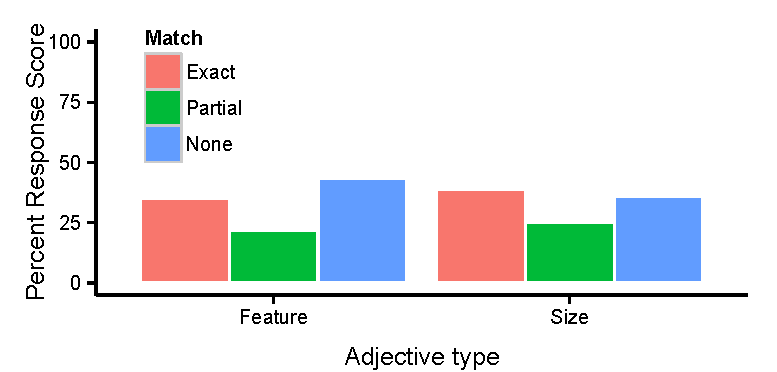
\includegraphics[width=6in]{figures/freeResponse_bars.pdf} 
    \caption{\label{fig:freeResponse} 4-year-olds� free responses about properties of other category members upon hearing a feature adjective (left) or size adjective (right).  Productions were coded as \emph{exact matches} if they were opposite to the referenced description, \emph{partial matches} if they were related to the referenced property but not a direct contrast, or \emph{no match} if they were unrelated to the referenced modifier. }
    %Error bars represent 95\% confidence intervals.} 
  \end{center} 
  % \vspace{-2.0ex} 
\end{figure}

 


\section{General Discussion}

Our three experiments give support that children are sensitive to not just \emph{what} speakers say, but \emph{how} they say it.  We used the case study of adjectives to investigate whether children infer that speakers' modified descriptions imply knowledge about relevant dimensions of contrast. In Experiment 1, we showed that by age 3.5, preschoolers reliably made contrast inferences from size and feature adjectives with the support of a contrastive linguistic framing (``This is a special kind of tibu'').  Unlike adults, 4-year-olds in Experiment 2 had difficulty making contrast inferences when the contrast framing was removed, although their performance increased after exposure to adjective contrasts before undergoing the experimental task. Our forced-choice design may have made it especially difficult for children in Experiment 2 to reason between two plausible competitors (a property \emph{contrast} versus a property \emph{match}) from a single word cue. When these competitors were removed in our open-ended design in Experiment 3, 4-year-olds spontaneously produced relevant property contrasts the majority of the time, indicating that they can infer implied contrast information from adjective use alone, but their ability to reason backwards about pragmatic implications of word choices is still developing. Altogether, our results suggest that preschoolers appreciate adjective choice as conveying socially-relevant information about other category members. 

%
%reason about whether they should select the property \emph{contrast} conveyed in one picture or the property \emph{match} conveyed in the other picture based .  
%
%
%These findings suggest that preschoolers can infer relevant alternatives implied by word choice information, but they may rely on the support of additional cues such as a contrastive linguistic framing before spontaneously generalizing to visual competitors in our forced-choice task.  Our forced-choice task in Experiment 2 may actually be an especially challenging context for children to inter contrast because they were required to select between two plausible competitors 
%
%
%hey were required to select between one item that represented the \emph{same} property as the one stated, and one that was the \emph{contrast}.  This 
%
% In Experiment 3, we used a free response paradigm to examine children�s inferences from adjective use without the constraints of the forced-choice task.  We found that, although 4-year-olds could produce any response of their liking, they spontaneously stated relevant contrast information more than half of the time.  Altogether, our results suggest preschoolers appreciate adjective choice as conveying contrast information about other category members. 

Although simple in design, our task required a fairly counterintuitive response: hearing a description and inferring its opposite. In other words, children needed to process the stated adjective and then select the picture that \emph{differed} from that description instead of the one that shared that property, even though both picture options were available. This task requires both pragmatic reasoning about how people use language, and also executive control to inhibit a matching bias to instead select the non-match.  We found that preschoolers nonetheless made these contrast inferences and robustness increased age, suggesting that they are reasoning backwards to infer contrast from speakers' word choices. Their sensitivity to the pragmatic implications of adjective use gives evidence that they are indeed processing information not just about what is stated explicitly, but also about what is culturally relevant to support such a description. 

Our studies contribute to the growing literature suggesting that children consider how and why evidence is generated to reason about the social world. By preschool age, children differentiate that random sampling conveys cues about the likelihood of distributions, while non-random sampling conveys social cues about preferences and pedagogical information \cite{xu2009, kushnir2010, butler2012}. In the domain of language, they appear to use descriptive choices to infer the implications of speakers' intended meaning to infer reference \cite<e.g.>{stiller2014}. Building on the \emph{alternatives hypothesis} that children's ability to compute implicatures relates to their recognition of linguistic alternatives \cite{barner2011}, they may need to accumulate experience with how cultural information about the world is conveyed before recognizing relevant opportunities for pragmatic inference. 


Most work to-date has focused on children's inferences about speakers' intended meaning in a referential context based on language use, and our work takes a novel approach by examining children's inferences about the state of the world that would lead a speaker to make particular production choices. While preschoolers show evidence of distinguishing generalizable knowledge from specific descriptions based on framing cues \cite{cimpian2009}, we extend these inferences to investigate children's intuitions about what world-states support contrastive descriptions.  In other words, we examine children's ability to reason about other category members not simply by generalizing the speaker's description (e.g. that hearing ``small tibu'' implies that all tibus are small), but rather by inferring property variability by pragmatic contrasts (that marking a tibu as ``small'' implies that others vary by size).  Our work suggests that children not only use modified descriptions to mark non-generic information, but they can also reason about implied alternatives specific to the adjective produced.
%Extending their understanding of rational agents and sampling \cite<e.g.>{xu2008, xu2009, gweon2010}, preschoolers may use the informativeness of word choices to consider the implied state of the world that might lead to those choices. Their sensitivity to statistical regularities in the world may help them expect that modified referents contrast with other category members along the stated property dimension (i.e. that ``big dog'' implies that dogs can vary by size).  Just as they can reason about likely sample to population of pingpong balls, language cues such as adjective use may implicitly convey cultural knowledge about the world.  In this way, word choices refer not just to references in the present (e.g. the big dog currently in sight), but also to contrasts with other possible contexts and category members (that this dog happens to be big, and others are smaller).     

%If children assume that speakers are being both rational and communicative, then they can take advantage of opportunities for inference wherever they recognize a speaker's choice to produce an utterance in one form over another.  Building on the hypothesis that children's abilities to compute implicatures relates to their ability to recognize linguistic alternatives \cite{barner2011}, children may need to accumulate experience with how cultural information about the world is conveyed before recognizing relevant opportunities for pragmatic inference. 


%Our case study of adjectives provides evidence that children are learning to process both explicit and implicitly conveyed information. Their increasing familiarity with opposite pairs leads them to robustly infer contrast with age given a supportive linguistic framing in Experiment 1 and with recency of exposure to contrasts in Experiment 2.  Without any constraints, they generated relevant alternatives on their own more than half of the time. The ability to infer culturally-implied knowledge may require both the recognition of production choices that imply alternatives and also what those particular alternatives are. 

Our work connects mechanisms of pragmatic inference, which have been well-studied in language development, with processes of social learning and generalization.  Children may need to accumulate experience with how cultural information about the world is conveyed before recognizing relevant opportunities for pragmatic inference. 
 If children assume that speakers are being both rational and communicative, then they can take advantage of opportunities for inference wherever they recognize a speaker's choice to produce an utterance in one form over another.  We show that children can figure out that naming a ``tall glorp'' implies that most glorps are shorter. The same mechanism might also allow them to infer (usefully) that the term ''cognitive scientist'' implies the existence of other types of scientists, or to infer (negatively) that ``female scientist'' implies that most scientists---at least in the mind of the speaker---are not female. Thus, pragmatic inferences of the type we study here may constitute an important mechanism of transmission for cultural knowledge.



\bibliographystyle{apacite2}
\bibliography{ADJ}

\end{document}
